\section{The Altered Period}

In the preceding section, we have learned that the computer is indeed limited and for every type of float there is an optimal increment for an approximation. To advance our understanding in this particular subject, let us modify the function and observe the effect on the error. Define
\begin{align*}
    g_j(x) := \frac{\sin(j x)}{x} \text{,}
\end{align*}
and we have the derivatives
\begin{align*}
    g_j'(x) &= \frac{j x \cos(jx) - \sin(jx)}{x^2} \\
    g_j''(x) &= \frac{(2 - j^2 x^2)\sin(jx) - 2 j x \cos(jx)}{x^3} \text{,}
\end{align*}
with \(j > 0\). Once again, we will evaluate these functions on the partitioned interval \(I = [\pi, 3\pi]\) with \(p = 1000\). But given \(g_j\), how does large and small \(j\) affect the error plot?

%%%
\begin{figure}[h!]
    \centering
    \begin{subfigure}[b]{0.49\linewidth}
        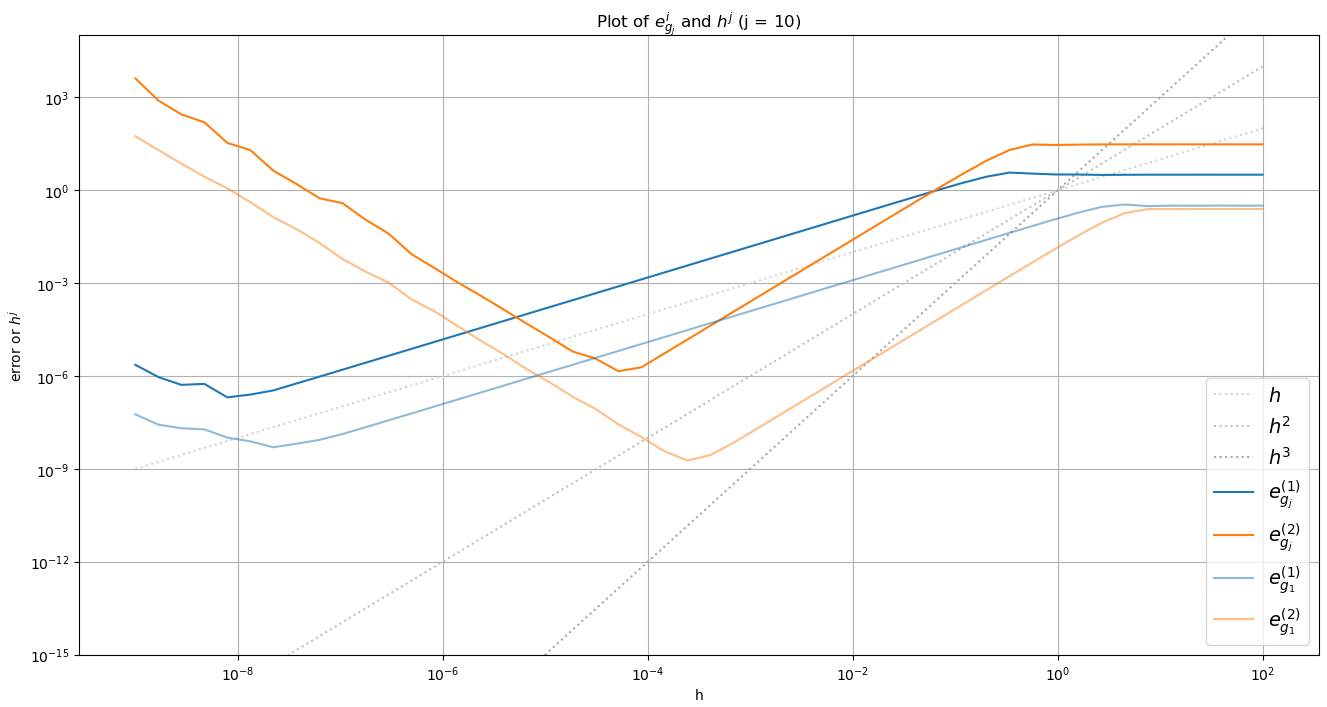
\includegraphics[width=\linewidth]{graphics/j_error_plot/big_j.png}
    \end{subfigure}
    \begin{subfigure}[b]{0.49\linewidth}
        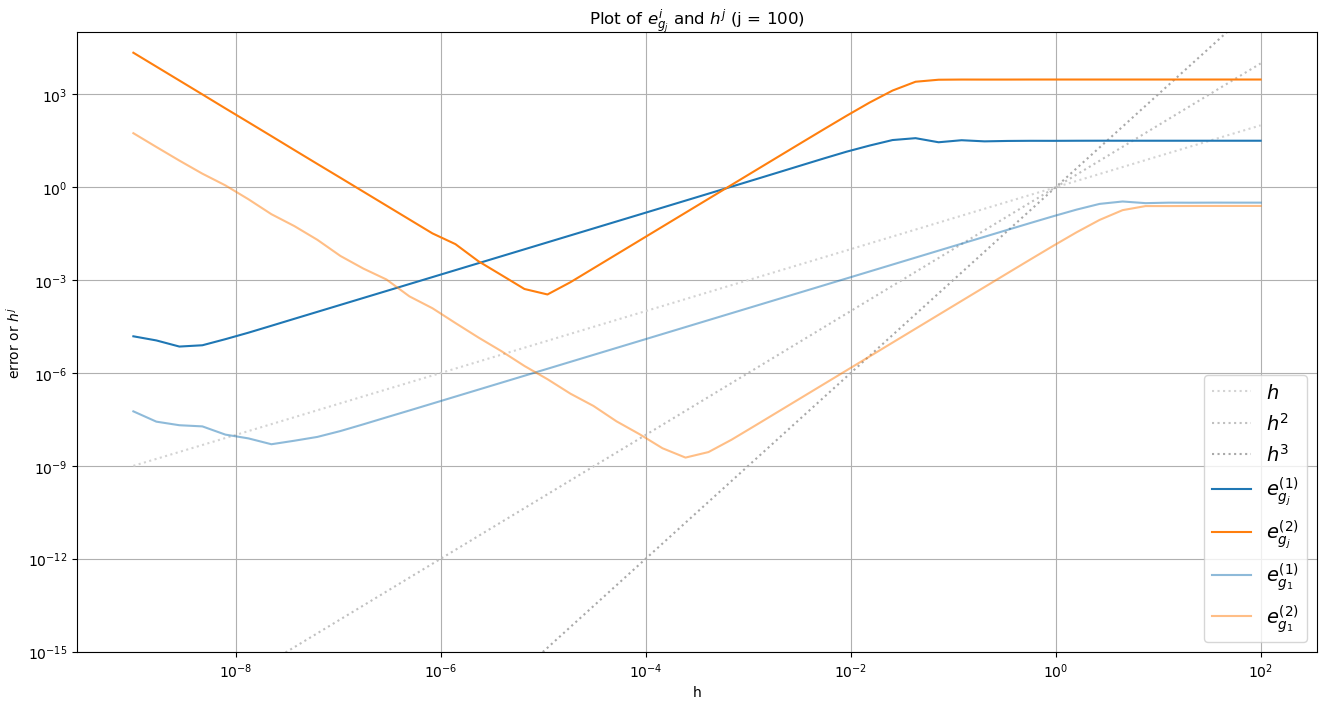
\includegraphics[width=\linewidth]{graphics/j_error_plot/large_j.png}
    \end{subfigure}
    \begin{subfigure}[b]{0.49\linewidth}
        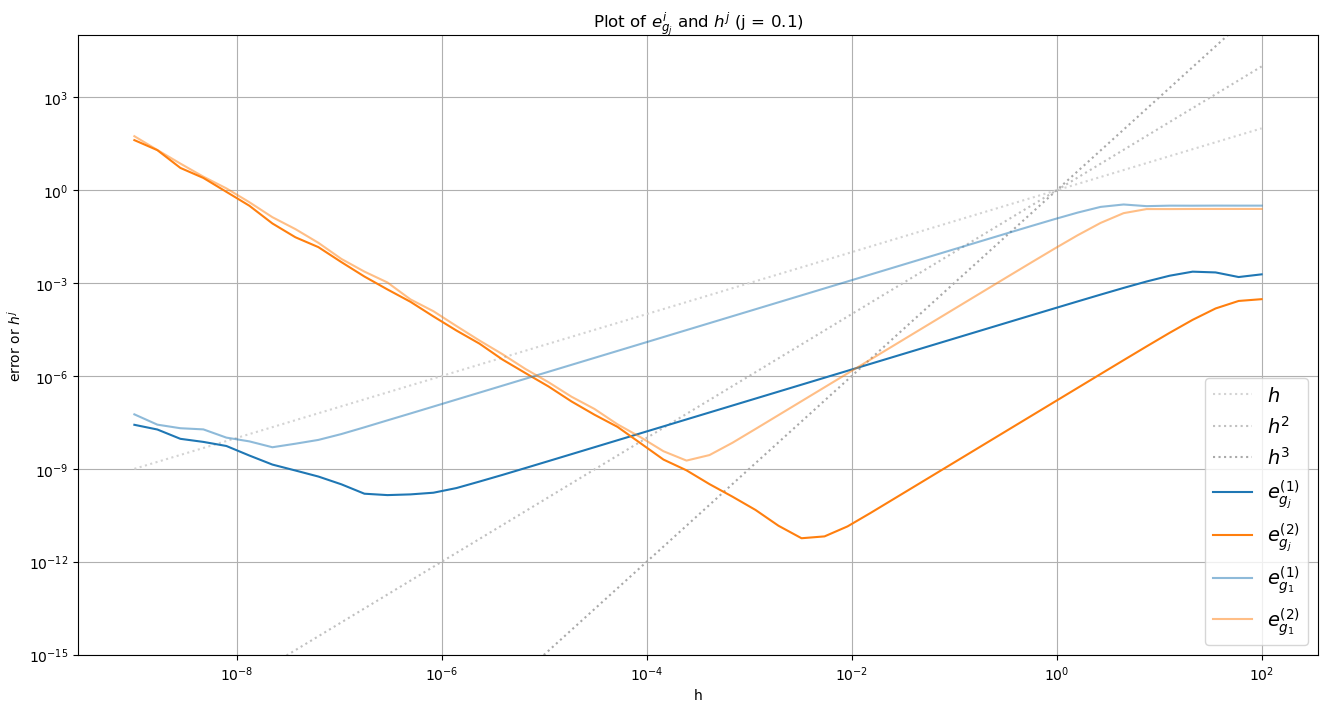
\includegraphics[width=\linewidth]{graphics/j_error_plot/small_j.png}
    \end{subfigure}
    \begin{subfigure}[b]{0.49\linewidth}
        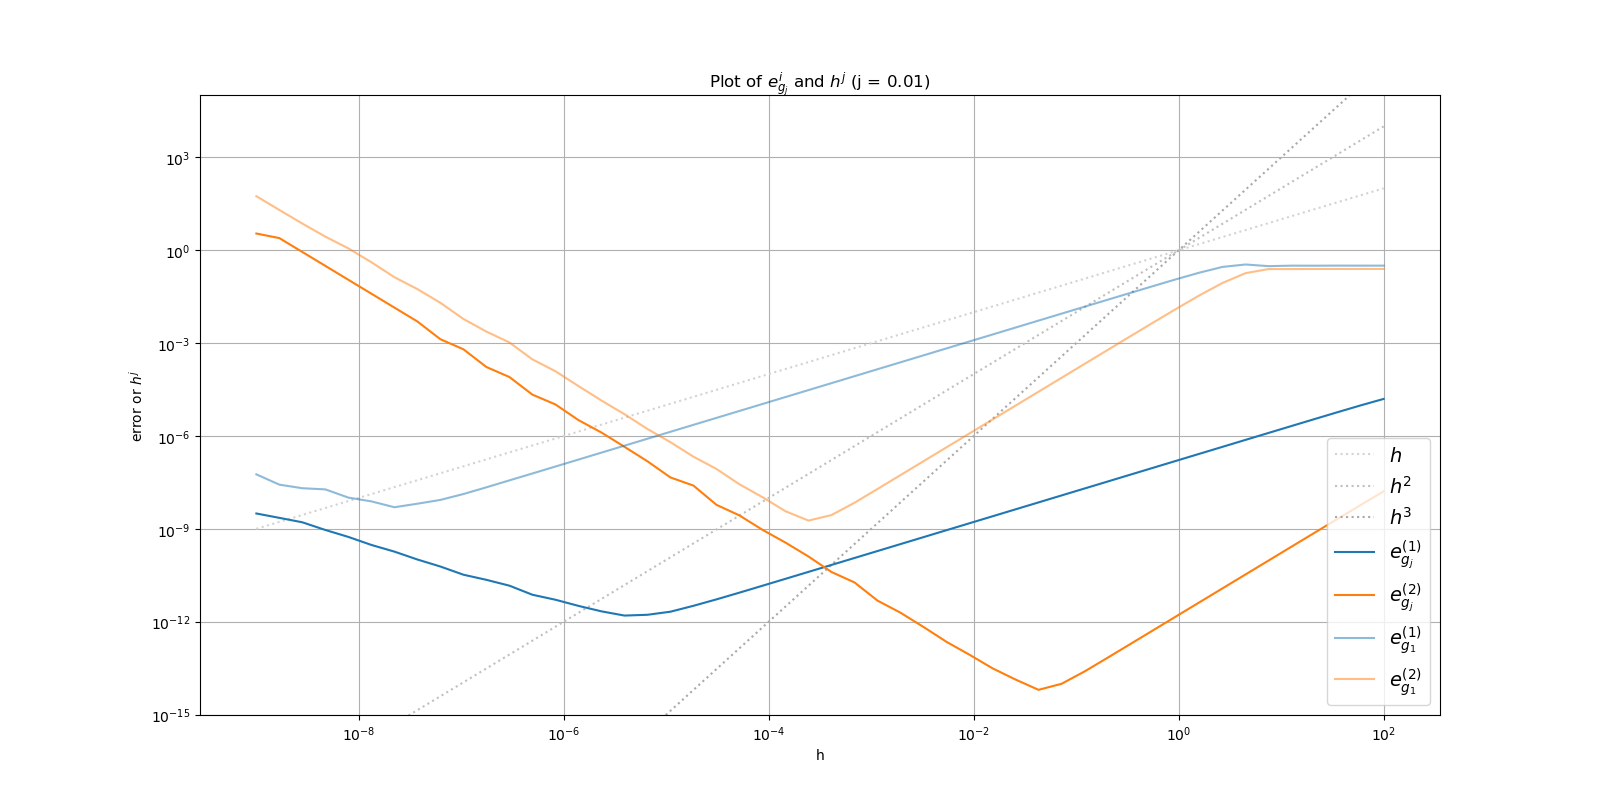
\includegraphics[width=\linewidth]{graphics/j_error_plot/tiny_j.png}
    \end{subfigure}
    \caption{The Error Plot with various j}
    \label{fig:exp2_j}
\end{figure}

In figure \ref{fig:exp2_j}, one can see that as \(j\) gets smaller, the error plot and in particular sweet spot of the increment for both \((D^{(1)}_h g_j)\) and \((D^{(2)}_h g_j)\) moves to bottom right. This means, that the optimal choice for \(h\) becomes larger and the approximation becomes slightly better. On the other hand, choosing big values for \(j\) moves the curve and the sweet spot of both errors to the top left which means that one needs a smaller \(h\) for the most optimal yet worse approximation.
Why does this movement of the sweet spot occur? To answer this question, we have to look at what \(j\) does in our function \(\sin(\cdot)\). \(j\) changes the period, the smaller the \(j\) the smaller the period and vice versa. Because \(g_j\) is once again a periodic function\footnote{A function \(f\) is periodic if there is a nonzero constant \(P \in \mathbb{R}\), such that \(f(x + P) = f(x)\) for all \(x\) in the domain.}, this property of periodicity is inherited from \(\sin(\cdot)\). If we now consider once again how the approximation is calculated, we had
\begin{align*}
    D^{(1)}_h (g_j) &= \frac{g_j(x + h) - g_j(x)}{h} \\
    D^{(2)}_h (g_j) &= \frac{g_j(x + h) - 2 g_j(x) + g_j(x - h))}{h^2}\text{.}
\end{align*}
We already know that the subtraction at the numerator is the source of imprecision. If \(j\) is small however, then \(g_j(x + h) - g_j(x)\) is also small (similar argumentation also applies for \(g_j(x + h) - 2 g_j(x) + g_j(x - h)\). This means, that even if \(h\) is comparatively large, the numerator of the approximation is still small. Therefore, the quotient of the approximation approaches the exact derivative for a larger \(h\) and more accurately if \(j \ll 1\) than for \(j = 1\). Conversely, if \(j\) is large, then even small change in \(h\) results in large difference at the numerator and we get an approximation for which smaller \(h\) is required for a worse approximation.